\chapter{Definition der Use-Cases} \label{Defintion der Use-Cases}

%kleine und mittlere \gls{Deployment}s... statt KMU. Bachelor-Arbeit war moving target
%Mein Ansatz: bis zu einer technischen Größenordnung ist das okay... Ansonsten Direct Connect oder Express Route
%Für kleine und mittlere \gls{Deployment}s (nicht KMU) -> keine kaufmännische sondern technologische Betrachtung
%Weniger Ebenen!

%"Qualitätssicherung": Warum haben sich die Erkenntnisse aus dem Proposal zur Arbeit geändert? Halbe Seit
 %Eine private Adressierung der Systeme ist noch nicht möglich, die Maschinen werden über die öffentlichen IPs aus dem Internet erreicht. Die Firma besitzt eine private Cloud
%ToDo: Genauer beschreiben, was beim Kunden schon zur Verfügung steht (Private Cloud) und dass das abstrahiert (vereinfacht) dargestellt wird


\section{Use Case 1: Basis mit Ende-zu-Ende-Konnektivität}\label{base-deployment}

%Use-Case 1: Ende-zu-Ende-Kommunikation, Beispiel Server
%Historisch gewachsen...
Es wird ein Basis \gls{Deployment} benötigt, um eine grundlegende Integration in die Firmeninfrastruktur zu ermöglichen. So ist die Grundannahme, dass der Kunde bereits Rechenressourcen in Selbstverwaltung (\glqq Private Cloud\grqq{}) besitzt. Weiterhin hat die Integration von Public Cloud-Diensten noch gar nicht oder nur testweise stattgefunden: Es wurden ein paar Maschinen hochgefahren und bestimmte Internetdienste installiert. Über eine tiefergehende Koppelung mit bestehender Infrastruktur hat der Kunde bisher keine Überlegungen angestellt.\\
Eine Hybrid Cloud besteht, wie bereits beschrieben, aus Public und Private Cloud. Da mit den beiden Public Clouds AWS und Azure gearbeitet wird, wäre hier bereits eine Fallunterscheidung notwendig: Private Cloud $\leftrightarrow$ Azure bzw. Private Cloud $\leftrightarrow$ AWS. Um sich diese Fallunterscheidung sparen zu können, soll ein Dreieck ausgerollt werden, bei dem jeder Punkt eine Cloud-Plattform darstellt.
%Weitere Vorteile ergeben sich später: Redundanz, einfaches Skalieren _zwischen_ Public Clouds
%Bild Basis \gls{Deployment}
Optimalerweise wird durch dieses \gls{Deployment} auch die Redundanz erhöht: Fällt eine Verbindung aus bspw. zwischen AWS und Azure, so können Datenpakete weiterhin über die Private Cloud geroutet werden.
%Bild Link Fail

%Kein NAT -> Ende-zu-Ende-Kommunikation _aller_ Teilnehmer

Der Use-Case soll als Grundaufbau für alle weiteren Use-Cases dienen und eine Ende-zu-Ende-Konnektivität für alle Teilnehmer garantieren. Das Dreieck aus AWS, Azure und Private Cloud wird fortan als \textit{Backbone} bezeichnet.

\begin{figure}[h]
  \centering
  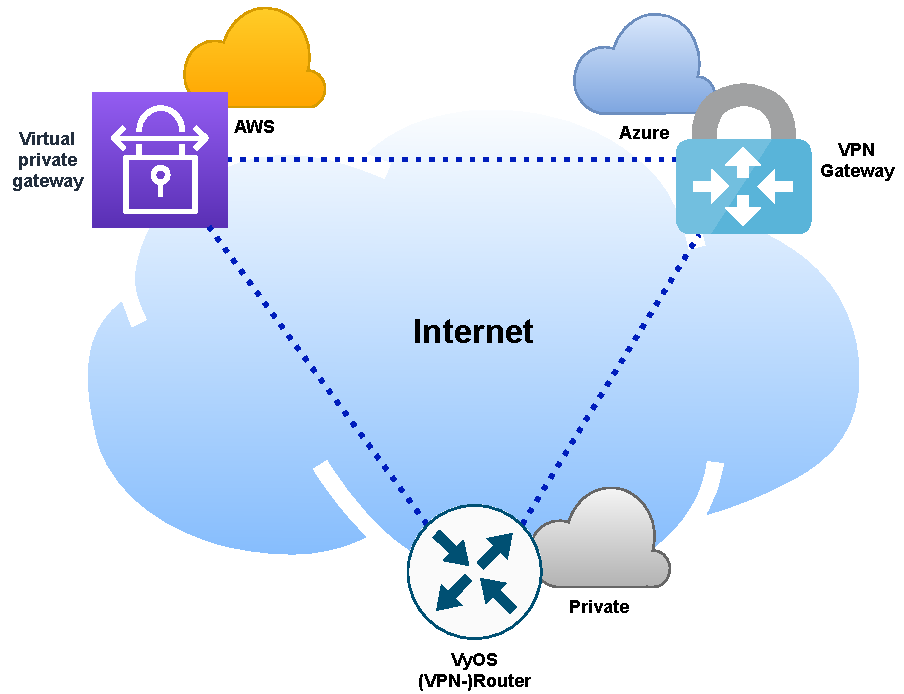
\includegraphics{Figures/Use-Case-1_Basis_Deployment.pdf}
  \caption{Use-Case 1: Dreiecks-Topologie für die Hybrid-Cloud (\glqq Backbone\grqq{})}
  \label{grafik:Use-Case-1_Basis_Deployment}
\end{figure}\FloatBarrier

\subsection{Vorauswahl geeigneter technischer Komponenten}
%PFS, AES Best Practices referenzieren
AWS und Azure bieten auf ihren Plattformen Unterstützung für Route-Based IPsec-Tunnel\cite[S.32]{awsvpn2021}. Darüber kann eine virtuelle Punkt-zu-Punkt zwischen zwei Standorten hergestellt werden und es kann innerhalb der Tunnel BGP gesprochen werden, um ein dynamisches Routing zu ermöglichen\cite[S. 18]{AlShawi2020} \cite[S. 74-79]{Toroman2019}. Gleichzeitig werden übertragene Daten verschlüsselt und dadurch Integrität und Vertraulichkeit geschützt.\\
Das dynamische Routing bietet den Vorteil, dass IPv4-Routen nicht manuell bei allen Gateways des Netzwerks bekannt gemacht werden müssen: Sobald ein Teilnehmer ein neues Netzwerkt kennt, wird dies via BGP den restlichen Teilnehmern bekannt gegeben.\\
%In technischen Grundlagen erwähnen: IaC, Provider, Module
%Mozilla Public License v2.0[2]
%Beispiel aus der Realität nennen: Switch - Kabel - Server
%MIT TECHNISCHEN GRUNDLAGEN ABGLEICHEN!!!
Für das automatisierte \gls{Deployment} der Infrastruktur eignet sich Terraform der Firma Hashicorp. Es besitzt eine Vielzahl an \textit{Resources} (u.a. Azure und AWS), welche es ermöglichen, Infrastrukturkomponenten \textit{reproduzierbar} bereitzustellen.\\
Darüber hinaus wird ein IPAM benötigt zur IPv4-Adressverwaltung. Die automatische Zuteilung von Adressbereichen darf nicht dazu führen, dass Adressbereiche mehrfach verteilt werden oder sich Adressbereiche überlappen. Gewählt wurde hier das Werkzeug phpIPAM\cite{phpipam2020}: Es lässt sich sehr gut mit Terraform integrieren, da ein entsprechender Provider zur Verfügung steht\cite{phpipamtf2020}.\\
Die VPN-Gateways, die das Backbone aufspannen, sind mit \textit{Virtual private gateway} bei AWS und \textit{VPN Gateway} bei Azure gesetzt. Dies sind die typischen \textit{Building-Blocks}, die von den Cloud-Providern für VPN-Verbindungen angeboten werden. Nur wenn sich im Laufe der Arbeit herausstellen sollte, dass diese Systeme nicht interoperabel sein sollten, wird versucht, Alternativen zu finden.\\
Als Router, der die Private Cloud repräsentiert, wurde ein VyOS Router gewählt. Dieser steht als Open Source zur Verfügung, es gibt allerdings auch bezahlten Support für Produktionsumgebungen. Der Router hat IPsec- und BGP-Unterstützung und besitzt ein Command Line Interface, über das Konfigurationen getätigt werden können. Eine REST-API steht ebenso zur Verfügung, aber diese ist zum Stand der Bachelor-Arbeit \textit{cutting edge} und eher dürftig dokumentiert\cite{vyosapi2021}. Ein nativer Terraform Provider steht nicht zur Verfügung.
Es soll pro Public Cloud eine virtuelle Maschine bereitgestellt werden, um die Ende-zu-Ende-Konnektivität zwischen den Standorten zu verifizieren.
Die Annahme ist, dass der VyOS-Router, das IPAM und eine virtuelle Maschine zum Testen in der Private Cloud bereits vorhanden sind. Diese Komponenten sind nicht Teil des (Terraform-)Deployments. Allerdings müssen Konfigurationsänderungen zum \gls{Deployment} geschehen.\\
Prinzipiell lassen sich viele Router-Modelle nutzen, insofern die Unterstützung für genannte Techniken (Route-based IPsec, BGP) vorhanden ist, bspw. CSR 1000V der Firma Cisco\cite{Durai2016}. Der offene VyOS Router bietet den Vorteil, dass keine Lizenzen für die Nutzung hinterlegt werden müssen, was in vielen Fällen manuelle Konfigurationen erfordert. Außerdem hätten erst einmal passende Lizenzen beschafft werden müssen, was u.U. zu Verzögerungen des Projekts geführt hätte.




%Kein NAT, da am Anfang evtl. einfacher, aber am Ende nur Ärger und Freischaltungen etc...

%Um den Anspruch der Automatisierung gerecht zu werden, ...
%Evaluationskriterien nummerieren
\subsection{Evaluationskriterien}\label{eval-kriterien-uc1}
Nach der Umsetzung wird evaluiert, ob das \gls{Deployment} folgender Kriterien erfolgreich war:
\begin{enumerate}
    \item IPv4-Adressbereiche werden im IPAM reserviert und mit AWS VPC und Azure VNET assoziiert. Test-Szenario: Zur Verifizierung werden die reservierten Adressbereiche mit den assoziierten verglichen.
    \item IPsec-Verbindungen werden zwischen allen VPN-Gateways aufgebaut. Test-Szenario: Dies kann mit einem Blick in die verschiedenen \textit{Dashboards} der Cloud-Plattformen bzw. CLI-Kommando (VyOS) verifiziert werden.
    %FIB in technischen Grundlagen?
    \item BGP-Sessions werden etabliert und Präfixe zwischen den Teilnehmern ausgetauscht. Die Routen müssen in der Routing-Tabelle sichtbar sein. Test-Szenario: Eine Testmaschine pro Site und Ping-Tests zwischen den Sites veranlasst werden.
    %Evtl. noch testen, ob Pings auch bei Verbindungsverlust funktionieren
    \item Die Präfixe sollten im Normalfall über verschiedene AS-Pfade sichtbar sein. Nur bei Verbindungsverlust sind Präfixe ausschließlich über einen AS-Pfad zu sehen. Test-Szenario analog zu Punkt 2.
    \item Verifizierung der Ende-zu-Ende-Konnektivität und einfache Bandbreitenmessungen. Test-Szenario: Ping-Tests und iPerf3-Messungen zwischen den Standorten.
\end{enumerate}
